\documentclass[11pt,twoside]{amsart}
\usepackage{/home/alex/.latex/stylesheet}
\usepackage{graphicx}
% \usepackage{multicol}
\usepackage{hyperref}
\usepackage{caption}
\usepackage{subcaption}
\graphicspath{ {./images/} }
\usepackage[backend=bibtex,style=numeric-comp,natbib=true]{biblatex}
\bibliography{paper}


\theoremstyle{theorem}
\newtheorem{theorem}{Theorem}
\newtheorem{corollary}[theorem]{Corollary}
\newtheorem{proposition}[theorem]{Proposition}
\newtheorem{lemma}[theorem]{Lemma}
\theoremstyle{definition}
\newtheorem{definition}[theorem]{Definition}
\newtheorem{example}[theorem]{Example}
\theoremstyle{remark}
\newtheorem{remark}[theorem]{Remark}

\title{Further Investigations into Schelling's Model}
\author{Alex Ledger}
\date{}
\pagestyle{headings}


\begin{document}
\maketitle
\tableofcontents

\newpage

\section{Introduction}
The goal of this paper is two fold. 
First, we wish to find where Schelling's model breaks down; that is, for what parameters does Schelling's model fail to exhibit the expected emergent behavior?
Second, we wish to add to the tools for analyzing the question: to what extent can we make conclusions about reality based on information provided by Schelling's model.
We assume the reader is familiar with the idea of complex systems, emergent behavior and cellular automata to the extent that one would learn in Mark Bedau's Philosophy of Computation course. 


\section{Review of Complex Systems, Emergent Behavior, Cellular Automata}
According to Aristotle, ``the whole is more than the sum of its parts.'' % THESIS P 19
This is according to modern memory, the first known description of a complex system.
The idea at its core does not get much more complicated that Aristotle's description: a complex system is a system where there are simple interactions on the micro level, but the simple interactions in aggregate give rise to more complex behavior at the macro level. 
We call the behavior at the macro level \emph{emergent behavior}.

The reason that we are intersted in complex systems is that they seem the be pervasive in the world: ecological systems, evolutionary systems, culture, and countless other places.
Then, if we are able to understand complex systems better, then perhaps we would be able to understand what is going on the world better. 

One method of going about this is to construct complex systems in a computational setting. 
An example of a class of complex systems designed in a computational setting is cellular automata.
Cellular automatas are models that take place on a discrete space, often of one or two dimensions. 
The examples I discuss are set on a two-dimensional discrete space; it is helpful to think of the space as a checkerboard. 
In an \emph{elementary cellular automata}, each cell can have two possible states: it can be empty or it can be occupied.
Then the state of a cell is updated based on the composition of its neighbors (e.g. how many of its neighbors are empty).
The cells are updated in discrete steps, and the rules here vary widely.
% ABOVE CITE THESIS PAGE 26 wolfram

More complex cellular automata have cells that can occupy more than two states. 
For example, in Schelling's model a cell can have take on three possible states: it can be empty, have a dime on it, or have a penny on it.
Naturally, the possible states can become more complex. 

It is important to note that not all cellular automata are complex systems. 
In fact, most of them aren't. 
The ones that are considered complex systems are members of class 4 cellular automata as defined by Wolfram. 
% CITE WOLFRAM
Class 4 cellular automata do not exhibit random activity, too much activity, too little activity, but what can be qualitatively described as a healthy amount of activity.
For more information on the types of cellular automata, see (TODO ADD WOLFRAM's PAPER)
In this paper, we will only be dealing with Class 4 cellular automata. 

\section{Review of Schelling's Model}
Schelling's model is a cellular automata presented by Schelling in a 1971 paper. 
It is meant to model segregation between groups of people of different interest. 

In the original model, Schelling uses pennies and dimes to represent two classes of people. 
For simplification of the idea, I simply refer to the two classes as white agents and black agents. 
Hence a cell can take on three possible states: it can be empty, be occupied by a white agent, or occupied by a black agent. 
Schelling randomly places black and white agents on a $8 \times 8$ checkerboard. 
Then Schelling stipulates that every white agent wants at least half of their neighbors to be white, and every black agent wants at least a third of their neighbors to be black.
Any agent whose preferences are not met is deemed unhappy. 
For each turn, select one unhappy agent at random and move the agent to the nearest cell such that the agent's preferences are met, i.e. the agent is happy.
Keep on moving agents until all agents are happy (it may be the case that this doesn't happen - we will address this in a second). 
After all of the agents are happy, we look at the organization of the agents on the board. 
What we see is that there are groups of white agents and separate groups of black agents: in a word, there is \emph{segregation}.

% address no equilibrium
In some cases, not all of the agents will become happy and the system will remain in flux. 
Despite this, we still witness segregation on the macro scale. 
For further discussion on the behavior exhibited by Schelling's model, we refer to reader to (TODO ADD CITE TO SCHELLING) (TODO ADD CITE TO THESIS).

For clarity, I offer a formal definition of neighbors.
\begin{definition}[Neighbors]
    The neighbors of an agent is the set of all agents in the $3 \times 3$ square surrounding the agent, where the agent's cell is in the center of the square. 
    We do not include the agent in the calculation of their neighbors. 
    % add figure here
\end{definition}

\section{My Work}
My goal in this section is to explore the question: for what parameters does Schelling's model faili to exhibit the expected emergent behavior?
In particular, I explore to what extent the emergent segregation in Schelling's model is dependent on moving an unhappy agent to the nearest cell whereby the agent becomes happy.
I investigate the implications of changing the moving procedure to having the agent go on a random walk and stopping the walk when (a) the agent finds an emtpy where they would be happy or (b) the agent visits more than 100 cells at which point the agent returns to their original position and remains unhappy.
I call the original model where the agents move to the nearest cell such that they are happy \emph{nearest}, and I call the model where the agents take a random walk \emph{random walk or rw}.

\subsection{What is a random walk?}
% TODO ADD IMAGE
Before moving forward, we introduce the notion and implementation of a random walk.
A random walk is, as the name suggests, where an agent moves around the board making deciding their path at random. 

% TODO FIX THE ALGORITHM FORMATTING
The algorithm is quite simple:
\begin{enumerate}
    \item Create set $S$ of all the adjacent cells to the current cell.
    \item Pick a random cell (uniform random) from set $S$.
    \item Move to that cell. 
    \item Repeat the above instructions until the conditions of the agent are met or the number of steps exceeds the alloted amount.
\end{enumerate}

For clarity, if the agent is residing in a cell in the middle of the board, there is a $\frac{1}{4}$ probability that the agent moves in particular cardinal direction.
If the agent on the board (but not a corner), the agent has a $\frac{1}{3}$ probability of moving to a particular cell of the three adjacent cell.
And if the agent is in a corner, the agent has a $\frac{1}{2}$ probabilty of moving to a particular cell of the two adjance cells.
Importantly, the agent \emph{always} moves; there is a zero probability that the agent stays in the same cell.

It could be the case that in a random walk, the agent moves back and forth between two cells until their $100$ steps are used up - although that is unlikely to occur. 
On the other hand, the agent could walk to every cell on the board, and unfortunately find that no cell makes them happy. 
More likely however, the agent explores some subset of the board at random, and searches for a happy cell.
I did not calculate it, but one certainly could analytically compute the expected number of unique visited cells in a random walk of $100$ steps (assuming the agent does not find a happy cell and end the walk early - that would complicate things).

\subsection{Metrics}
We used two methods for summarazing a state. 
The first is a metric called average similarity. 
We first compute the similarity of each individual agent, this is defined as
\[ \text{similarity(agent)} = \frac{\text{\# neighbors of same race as agent}}{\text{\# neighbors}} \]
Then we compute the average similarity for a state by averaging the similarity of the agents:

TODO MAKE BIG SUM?
\[\text{average similarity(state)} = \frac{\sum_{\text{agent on board}} \text{similarity(agent)}} {\text{\# total agents}} \]
The second metric is called average happiness, is computed:
\[ \text{average happiness(state)} = \frac{\text{\# happy agents}}{\text{\# total agents}} \]
Both average similarity and average happiness are ratios, that is their values are between 0 and 1. 
Moreover, both values, by their nature of being ratios, are largely invariant to the fixed parameters of Schelling's model. 
However, the values do correlate. Since agents in Schelling's model do have a preference to be near agents like themselves, it is expected that as agents become happy, average similarity increases. 

\subsection{Preferences}
The preferences refers the agents' desired composition of neighbors.
If an agent has a preference ratio of $0.5$, then the agent wants at least half of their neighbors to be of the same race as them.
Alternatively if an agent has a preference ratio of $0.3$, then the agent wants at least $30\%$ of their neighbors to be of the same race as them.
Preferences is the parameters I swept over, in attempt see how the combination of preferences and the moving procedure changed the macro behavior of the system, in the particular the average similarity.
I kept the preferences of the black agents constant at $0.3$ through all of the trials.
I changed the preferences of the white agents. 
The preferences for white people that I tested were $0.3, 0.4, 0.5, 0.6$, and $0.7$. 
The preferences can be understood with the following intuition: as the preference ratio increases, the agent becomes selective about their neighbors, i.e. the agent becomes more racist. 

The preferences are preset before the model begins running; the preferences of agents do not change over time. 


\subsection{Procedure}
We computed a board state randomly using the following algorithm: 
\begin{enumerate}
    \item Initialize the each cell as empty.
    \item For each cell, pick an element of $\{0,1,2\}$ uniformly random. If $0$, leave the cell empty. If $1$, put a white person in the cell, if $2$ put a black in the cell.
\end{enumerate}
I ran the nearest model and the random walk model using the same randomly contructed initial state. 
After moving an agent, I recorded the average similarity and average happiness. 
For each set of preferences, I did 25 trials of the nearest simulation and the random walk simulation.

\subsection{Results}
As mentioned, I did 25 trials of each model for each set of preferences. 
For each set of 25 trials, I computed the average of the average similarity for each iteration. 
I did likewise for the average happiness. 

TODO FORMAT GRAPHICS - SEARCH ONLINE
    \begin{figure}
        \begin{subfigure}[b]{0.3\textwidth}
            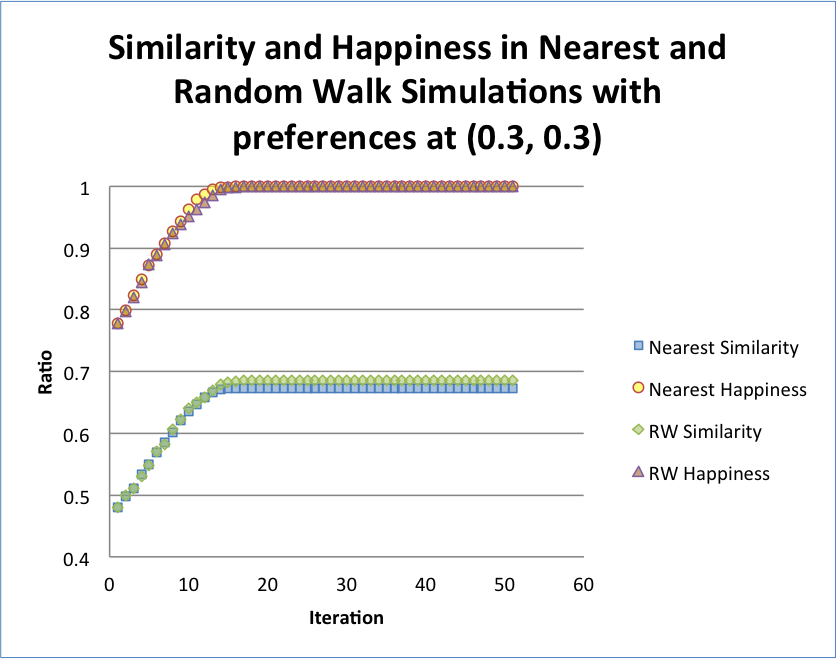
\includegraphics[scale=0.35]{3_3.png}
        \end{subfigure}

        \begin{subfigure}[b]{0.3\textwidth}
            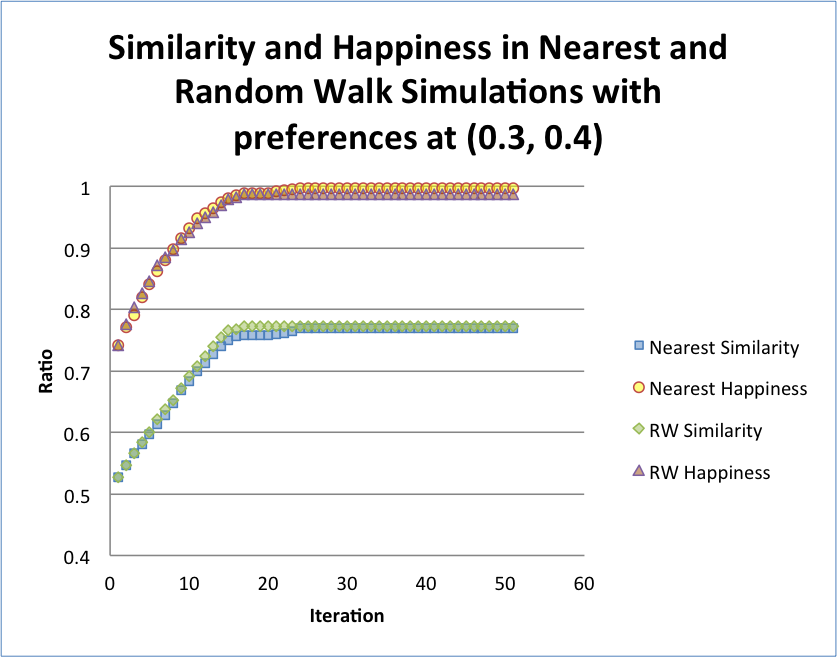
\includegraphics[scale=0.35]{3_4.png}
        \end{subfigure}
    \end{figure}

    \begin{figure}
        \begin{subfigure}[b]{0.3\textwidth}
            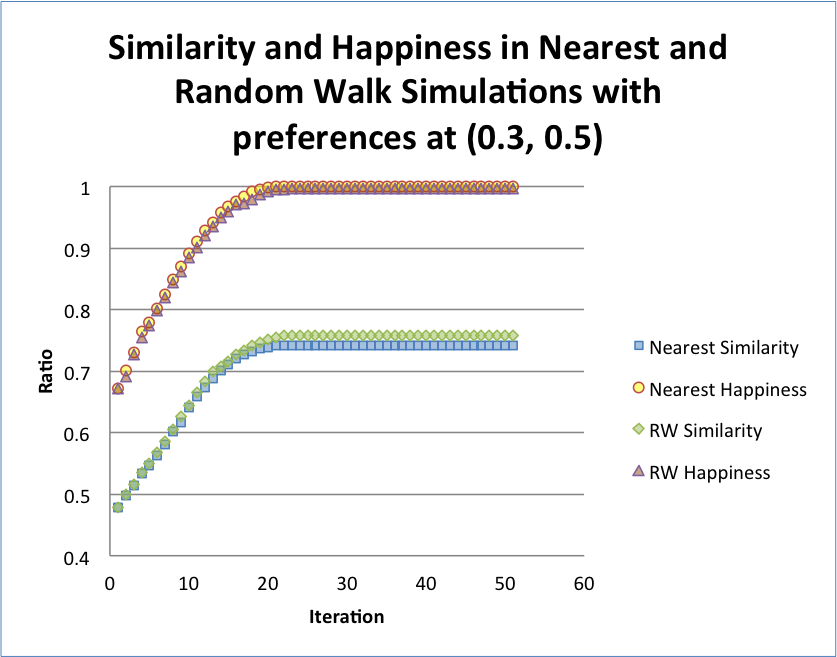
\includegraphics[scale=0.35]{3_5.png}
        \end{subfigure}

        \begin{subfigure}[b]{0.3\textwidth}
            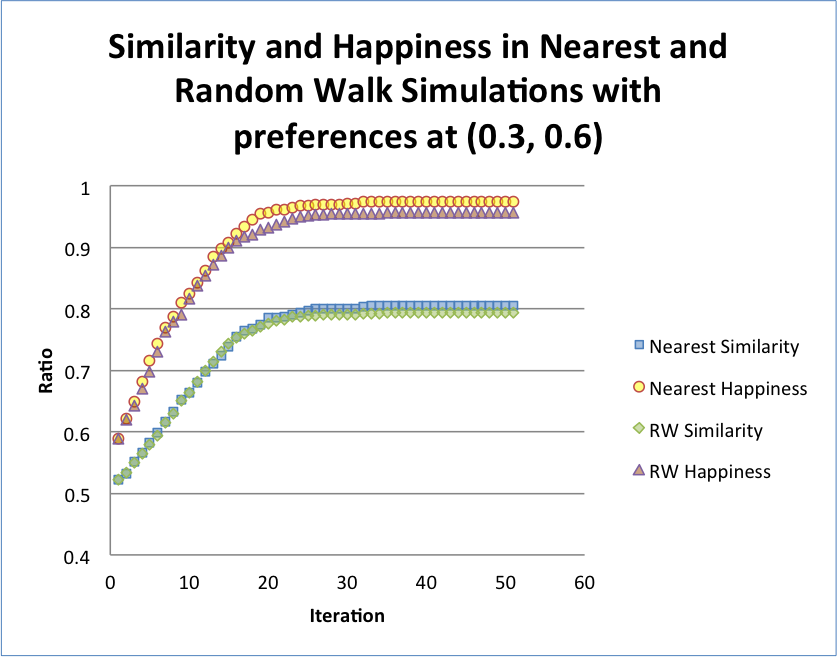
\includegraphics[scale=0.35]{3_6.png}
        \end{subfigure}
    \end{figure}

    \begin{figure}
        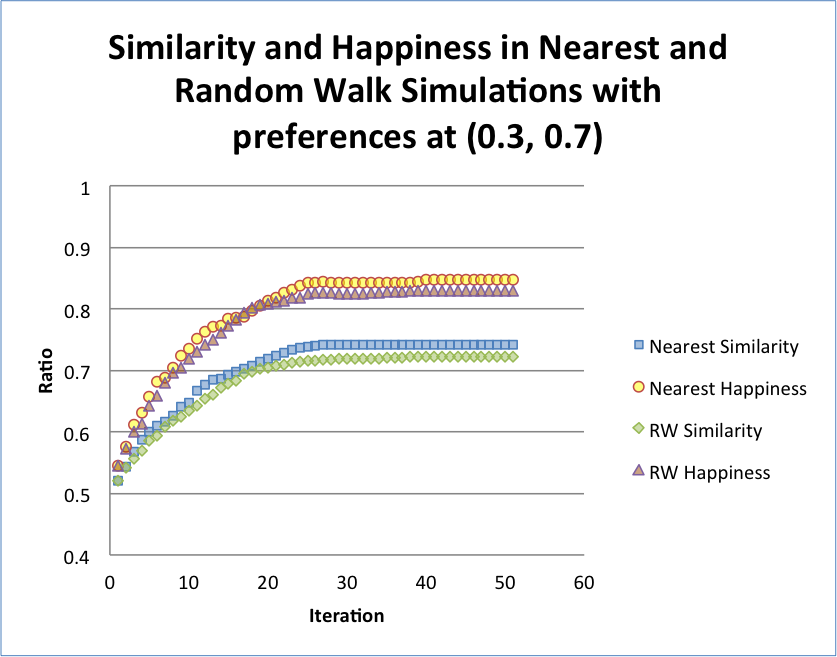
\includegraphics[scale=0.35]{3_7.png}
    \end{figure}

NOTE: in retrospect, I should have computer the standard deviation. I may do that when I have time next week.

\subsection{Analysis of results}
The results strongly suggest that there is not difference between the random walk model and the nearest model, insofar as the only parameter changing is the neighbor preferences of the whites. 
We expected that the the random walk model would converge more slowly the its final average similarity more slowly than the nearest model, but the rates of convergence are similar. 
TODO DIDN'T FINISH THIS

% Should have made max number of steps smaller


\subsection{A list of the parameters in Schelling's model}
    %This definition can be altered by input parameters. Instead of considering the $3 \times 3$ square, we could consider the $x \times x$ square, where $x$ is defined globally.
    \begin{enumerate}
        \item Boundary Conditions
        \item Neighborhood size or vision
        \item Perturb the system: in many biological models, they add random noise to make the model more realistic. 
            Examples of this in Schelling's model are:
            \begin{enumerate}
                \item moving happy agents randomly
                \item Removing and adding agents randomly
                \item Switching the race of a random agent
            \end{enumerate}
        \item Change preferences of models over time based on composition of environment. 
        \item Incoroporate an agent's memory. Maybe someone who lived in mixed race environment for a while will be less racist. And vice versa.
    \end{enumerate}
\section{Analysis}

\printbibliography

\end{document}
